\chapter{Introducción General}
\label{chap:introduccion}

El presente trabajo de graduación se desarrolla en el marco de la Facultad de Ciencias Exactas y Tecnología (FACET) de la Universidad Nacional de Tucumán (UNT). La FACET procesa un volumen constante de documentación administrativa y académica que requiere de mecanismos de validación y firma por parte de sus autoridades y personal docente.

\section{Descripción del Problema}
\label{sec:problematica}

Históricamente, el flujo de trabajo para la firma de documentos en la institución ha sido manual y descentralizado, con ineficiencias que dificultan el trabajo diario del personal académico.

El proceso actual comienza cuando un usuario necesita firmar un documento. Típicamente, debe descargar el archivo, firmarlo con alguna herramienta externa, guardar una copia y enviarla por correo electrónico al siguiente responsable. Este ciclo se repite hasta conseguir todas las firmas. El proceso se describe mediante un diagrama de flujo en la Figura~\ref{fig:flujo_proceso_firma_actual}, y genera los siguientes problemas:

\begin{itemize}
    \item Tiempo Administrativo: el usuario invierte tiempo en tareas repetitivas (descargar, buscar una herramienta de firma, procesar el archivo y volver a enviarlo) en lugar de realizar la acción de manera inmediata y centralizada.
    \item Errores Humanos: es común que se pierdan hilos de correos, se olviden archivos adjuntos o que los usuarios firmen en lugares incorrectos por no tener una guía visual clara en el documento.
    \item Falta de Trazabilidad: cada firmante posee una versión intermedia del documento en su dispositivo. No existe un registro centralizado que indique cuándo firmó cada persona (fecha y hora), ni un mecanismo que asegure el orden secuencial de las firmas, lo que dificulta saber en qué etapa exacta se encuentra el trámite.
    \item Uso Ineficiente del Almacenamiento: al no existir un repositorio único, ese archivo se replica innecesariamente y ocupa espacio tanto en los servidores de correo como en el almacenamiento local de cada usuario.
\end{itemize}

\begin{figure}[H]
    \centering
    {\setlength{\fboxsep}{6pt}%
    \colorbox{black}{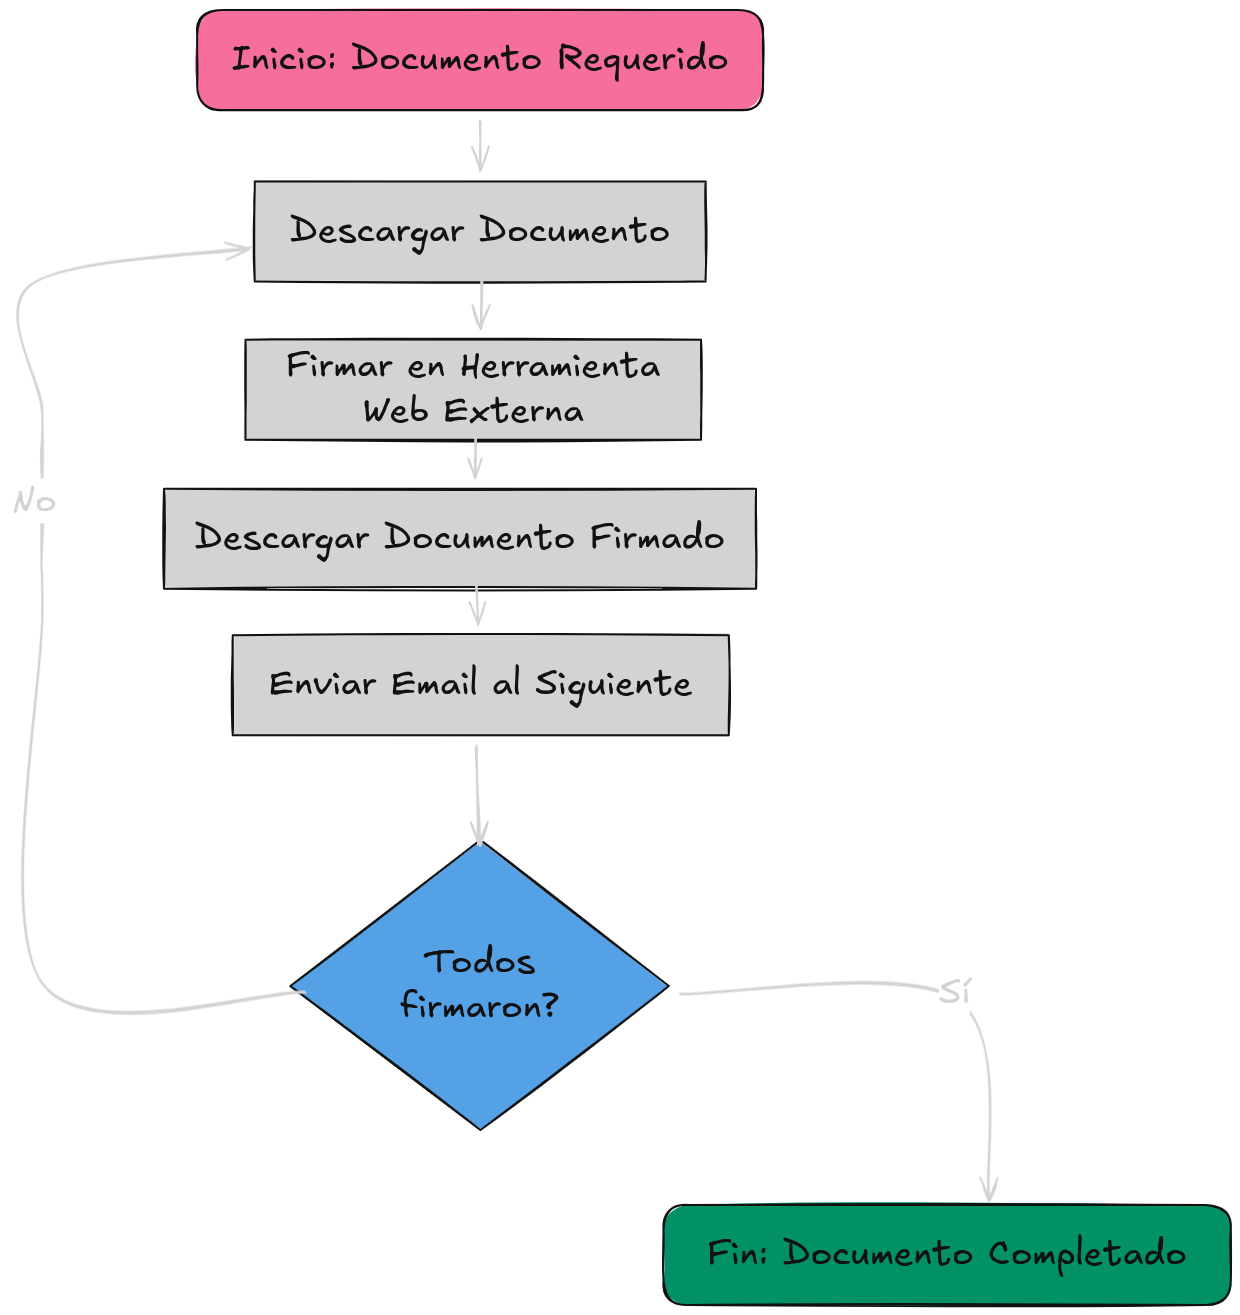
\includegraphics[width=0.62\textwidth]{figuras/capitulo1/diagrama-flujo_proceso-firma-actual.png}}}
    \caption[Flujo actual del proceso de firma]{Diagrama de flujo del proceso actual de firma de documentos en la facultad.}
    \label{fig:flujo_proceso_firma_actual}
\end{figure}

\section{Motivación y Justificación}
\label{sec:motivacion}

Este trabajo se propone transformar el proceso manual y fragmentado descrito en la sección anterior en un flujo automatizado, aprovechando la infraestructura tecnológica con la que ya cuenta la facultad.

Frente a servicios externos con costos recurrentes elevados, una solución interna permite optimizar el uso del hardware, los sistemas de almacenamiento y la red institucional. El modelo de gestión propuesto organiza el ciclo de vida del documento en cuatro etapas:

\begin{itemize}
    \item Carga única: el usuario (docente, alumno, personal de la facultad o tercero) sube el archivo PDF al sistema una sola vez.
    \item Definición de parámetros: se establecen los firmantes, el orden de las firmas y la ubicación visual de cada una en el documento.
    \item Orquestación automática: el sistema asume la gestión del proceso, enviando notificaciones, administrando los turnos y recolectando las firmas de forma ordenada.
    \item Resultado trazable: se genera un documento final único que contiene todas las firmas, almacenado de forma centralizada y con un registro de fecha y hora de cada intervención.
\end{itemize}

\section{Objetivos y Alcance del Trabajo}
\label{sec:objetivos_alcance}

\subsection{Objetivo General}
Diseñar, implementar y desplegar una solución ``llave en mano'' para la gestión y firma electrónica de documentos PDF en la facultad, definiendo la infraestructura y los procedimientos necesarios para su operación y mantenimiento.

\subsection{Objetivos Específicos}
\begin{itemize}
    \item Evaluar las alternativas de código abierto mediante un estudio comparativo, a fin de seleccionar la solución que mejor se adapte a la organización de la facultad y a su integración con los servicios institucionales de identidad y almacenamiento.
    \item Diseñar la arquitectura de despliegue, configurar la infraestructura de virtualización, red y almacenamiento, y las políticas de respaldo y retención.
    \item Validar la solución técnica mediante una prueba piloto con usuarios reales, asegurando que la herramienta responda correctamente al flujo de trabajo propuesto.
    \item Elaborar el manual de mantenimiento y los procedimientos que garanticen la transferencia de conocimiento y la continuidad del servicio.
\end{itemize}

\subsection{Alcance y Limitaciones}
Este trabajo se centra en las tareas de infraestructura y administración de sistemas. El alcance comprende las siguientes áreas técnicas:

\begin{itemize}
    \item Análisis de la topología de red existente de la facultad, desde el \textit{reverse proxy} perimetral hasta el entorno de virtualización Proxmox y el contenedor LXC donde operan Coolify y Traefik.
    \item Despliegue contenerizado de la plataforma y de sus servicios auxiliares como contenedores Docker administrados por Coolify, ejecutados sobre un contenedor LXC aprovisionado por la facultad en Proxmox.
    \item Integración con el servidor de almacenamiento de objetos TrueNAS/MinIO, incluyendo la resolución de la conectividad necesaria entre la red privada de Docker y la red institucional.
    \item Configuración de la autenticación mediante Google OAuth 2.0, delegando la verificación de identidad al dominio institucional de Google Workspace.
    \item Integración con un servicio externo de \textit{relay} SMTP para el envío de notificaciones transaccionales del sistema.
    \item Definición de políticas de respaldo y retención orientadas a la preservación de los datos transaccionales y los documentos firmados.
    \item Habilitación del acceso web cliente-servidor, garantizando la operabilidad de la plataforma desde navegadores estándar (escritorio y móviles) sin requerir instalación de software en los equipos.
\end{itemize}

Se establecen las siguientes limitaciones:

\begin{itemize}
    \item El trabajo no incluye el desarrollo de software de aplicación desde cero, sino la implementación, integración y optimización de herramientas de código abierto existentes para cumplir con los requisitos de la facultad.
    \item El hardware disponible en el servidor (procesadores Xeon E5620 sin soporte para instrucciones AVX/AVX2) impone un límite a la versión de las imágenes Docker utilizables, lo que restringe la plataforma a Documenso~v2.1.0. Este aspecto se documenta en el Capítulo~\ref{chap:diseno_implementacion}.
    \item El certificado de firma utilizado es autofirmado y no posee validez ante terceros externos, por lo que el sistema se clasifica legalmente como firma electrónica conforme a la Ley 25.506.
\end{itemize}

\section{Estado del Arte}
\label{sec:estado_arte}

El análisis inicial del sector permitió identificar una marcada diferencia entre las plataformas comerciales de tipo SaaS (\textit{Software as a Service}) y las alternativas de código abierto. Si bien el mercado comercial ofrece herramientas robustas, los costos de licenciamiento y la dependencia respecto de servicios externos motivaron el descarte de soluciones propietarias para la facultad.

Las soluciones líderes en el mercado se comercializan mediante planes de suscripción con costo recurrente, generalmente estructurados por usuario o por nivel de servicio, lo que resulta económicamente inviable para una institución pública en el contexto actual. En la Tabla \ref{tab:comparativa_saas} se detallan los costos de los proveedores más relevantes.

\begin{table}[H]
    \centering
    \begin{tabular}{l c}
        \toprule
        Proveedor & Costo por Usuario (USD/mes) \\
        \midrule
        DocuSign \cite{docusign_pricing} & \$25.00 \\
        Dropbox Sign \cite{dropbox_sign_pricing} & \$25.00 \\
        Adobe Sign \cite{adobe_sign_pricing} & \$22.19 \\
        \bottomrule
    \end{tabular}
    \caption[Comparativa de costos de soluciones SaaS]{Comparativa de costos de soluciones SaaS de firma electrónica.}
    \label{tab:comparativa_saas}
\end{table}

Considerando el escenario más económico entre los proveedores analizados (\$22,19 USD por licencia, Adobe Sign según la Tabla~\ref{tab:comparativa_saas}), la Ecuación~\eqref{eq:costo_anual_saas} cuantifica el costo anual proyectado para un grupo de apenas 20 usuarios, resultado que sigue siendo significativo para el presupuesto de una institución pública:

\begin{equation}
    \label{eq:costo_anual_saas}
    \text{Costo Anual} = 20 \text{ usuarios} \times 22{,}19 \text{ USD} \times 12 \text{ meses} = 5.325{,}60 \text{ USD}
\end{equation}

El ahorro en licencias que se logra con una solución de código abierto no es absoluto: al optar por un modelo \textit{on-premise}, la facultad asume la responsabilidad de garantizar la disponibilidad del servicio, el mantenimiento de los servidores y la seguridad de la red y el almacenamiento ---tareas que en una solución comercial quedarían delegadas en el proveedor---. Como contrapartida, la adopción de código abierto permite reducir costos recurrentes, preservar la documentación dentro de la infraestructura de la UNT y desarrollar capacidades técnicas propias. La implementación realizada establece, además, una base operativa para futuras iniciativas de digitalización dentro de la facultad.

\subsection{Alternativas de Código Abierto (\textit{Open Source})}
\label{subsec:alternativas_opensource}

Habiendo descartado las soluciones comerciales por su inviabilidad económica, la investigación se centró en plataformas de firma electrónica de código abierto que permitieran un despliegue \textit{Self-Hosted}. El análisis del estado del arte arrojó dos alternativas principales con un nivel de madurez apto para producción: DocuSeal y Documenso.

Ambas plataformas se distribuyen bajo la licencia de código abierto AGPL-3.0 y ofrecen la funcionalidad base de firma electrónica. Sin embargo, el análisis de sus características técnicas y de licenciamiento reveló diferencias relevantes para el contexto universitario, resumidas en la Tabla \ref{tab:comparativa_opensource}.

\begin{table}[H]
    \centering
    \small
    \begin{tabularx}{\textwidth}{X X X}
        \toprule
        Característica & Documenso (AGPL Core) & DocuSeal (AGPL Core) \\
        \midrule
        Gestión de Roles (RBAC) & \checkmark Incluido & $\times$ Bloqueado (Solo PRO) \\
        Inicio de sesión con Google OAuth & \checkmark Incluido & $\times$ Bloqueado (Solo PRO) \\
        Personalización Visual (Branding) & \checkmark Incluido & $\times$ Bloqueado (Solo PRO) \\
        \textit{Stack} Tecnológico & Remix, Prisma, PostgreSQL & Ruby on Rails, PostgreSQL \\
        \bottomrule
    \end{tabularx}
    \caption[Comparativa de plataformas de código abierto]{Comparativa de características en versiones de código abierto.}
    \label{tab:comparativa_opensource}
\end{table}

La versión comunitaria de DocuSeal restringe funcionalidades empresariales a la edición Pro \cite{docuseal}. La carencia de control de acceso basado en roles implica que, por defecto, todos los usuarios creados en la plataforma posean privilegios de administrador. Esta limitación compromete la seguridad de los documentos y hace inviable su adopción en un entorno institucional de múltiples usuarios.

Documenso cuenta, además, con una comunidad activa. Durante el despliegue, los intercambios mantenidos en su servidor de Discord resultaron útiles para identificar soluciones a problemas frecuentes y destrabar inconvenientes de instalación y operación.

Por estos motivos, se seleccionó Documenso como la plataforma definitiva para el trabajo. La decisión se apoya en tres criterios técnicos que resuelven las necesidades de la facultad:

\begin{enumerate}
    \item Seguridad e Identidad: soporte nativo para la integración con Google OAuth, lo que permite utilizar las cuentas institucionales \texttt{@herrera.unt.edu.ar} dentro del esquema de autenticación ya administrado por la universidad.
    \item Gestión Organizacional: la plataforma incluye una estructura de ``Equipos'' (\textit{Teams}) que permite mapear fielmente el organigrama jerárquico de la institución. Es posible instanciar una organización central (FACET) y subdividirla en equipos departamentales (como el DEEC o el Departamento de Física), aislando los documentos y plantillas de cada área.
    \item Ecosistema de Infraestructura: compatibilidad nativa con servidores de almacenamiento de objetos S3 (como MinIO) y con servicios de \textit{relay} SMTP para el envío de notificaciones transaccionales del flujo de firma.
\end{enumerate}

Documenso ofrece una solución sin costos de licenciamiento y con capacidad de crecimiento, sobre la cual se diseña la arquitectura que se detalla en los capítulos posteriores.
